\subsection{x86}

\subsubsection{x86 + MSVC}

Имеем в итоге функцию \TT{f\_signed()}:

\lstinputlisting[caption=\NonOptimizing MSVC 2010]{patterns/07_jcc/simple/signed_MSVC.asm}

\myindex{x86!\Instructions!JLE}
Первая инструкция \JLE значит \IT{Jump if Less or Equal}. 
Если второй операнд больше первого или равен ему, произойдет переход туда, где будет следующая проверка.

А если это условие не срабатывает (то есть второй операнд меньше первого), то перехода не будет, 
и сработает первый \printf.

\myindex{x86!\Instructions!JNE}
Вторая проверка это \JNE: \IT{Jump if Not Equal}.
Переход не произойдет, если операнды равны.

\myindex{x86!\Instructions!JGE}
Третья проверка \JGE: \IT{Jump if Greater or Equal}\EMDASH{}переход 
если первый операнд больше второго или равен ему.
Кстати, если все три условных перехода сработают, ни один \printf не вызовется. 
Но без внешнего вмешательства это невозможно.

Функция \TT{f\_unsigned()} точно такая же, за тем исключением, что используются инструкции 
\JBE и \JAE вместо \JLE и \JGE:

\lstinputlisting[caption=GCC]{patterns/07_jcc/simple/unsigned_MSVC.asm}

\myindex{x86!\Instructions!JBE}
\myindex{x86!\Instructions!JAE}
Здесь всё то же самое, только инструкции условных переходов немного другие:

\JBE\EMDASH{}\IT{Jump if Below or Equal} и \JAE\EMDASH{}\IT{Jump if Above or Equal}.
Эти инструкции (\JA/\JAE/\JB/\JBE) 
отличаются от \JG/\JGE/\JL/\JLE тем, что работают с беззнаковыми переменными.

\myindex{x86!\Instructions!JA}
\myindex{x86!\Instructions!JB}
\myindex{x86!\Instructions!JG}
\myindex{x86!\Instructions!JL}
\myindex{Signed numbers}
Отступление: смотрите также секцию о представлении знака в числах ~(\myref{sec:signednumbers}).
Таким образом, увидев где используется \JG/\JL вместо \JA/\JB и наоборот, 
можно сказать почти уверенно насчет того, 
является ли тип переменной знаковым (signed) или беззнаковым (unsigned).

Далее функция \main, где ничего нового для нас нет:

\lstinputlisting[caption=\main]{patterns/07_jcc/simple/main_MSVC.asm}

\clearpage
\myparagraph{x86 + MSVC + \olly}
\myindex{\olly}
\myindex{x86!\Registers!\Flags}

Если попробовать этот пример в \olly, можно увидеть, как выставляются флаги.
Начнем с функции \TT{f\_unsigned()}, которая работает с беззнаковыми числами.

В целом в каждой функции \CMP исполняется три раза, но для одних и тех же аргументов, 
так что флаги все три раза будут одинаковы.

Результат первого сравнения:

\begin{figure}[H]
\centering
\myincludegraphics{patterns/07_jcc/simple/olly_unsigned1.png}
\caption{\olly: \TT{f\_unsigned()}: первый условный переход}
\label{fig:jcc_olly_unsigned_1}
\end{figure}

Итак, флаги: C=1, P=1, A=1, Z=0, S=1, T=0, D=0, O=0.
Для краткости, в \olly флаги называются только одной буквой.

\olly подсказывает, что первый переход (\JBE) сейчас сработает.
Действительно, если заглянуть в документацию от Intel, 
(\myref{x86_manuals}) прочитаем там, что \JBE срабатывает в случаях если CF=1 или ZF=1.
Условие здесь выполняется, так что переход срабатывает.

\clearpage
Следующий переход:

\begin{figure}[H]
\centering
\myincludegraphics{patterns/07_jcc/simple/olly_unsigned2.png}
\caption{\olly: \TT{f\_unsigned()}: второй условный переход}
\label{fig:jcc_olly_unsigned_2}
\end{figure}

\olly подсказывает, что \JNZ сработает.
Действительно, \JNZ срабатывает если ZF=0 (zero flag).

\clearpage
Третий переход, \JNB:

\begin{figure}[H]
\centering
\myincludegraphics{patterns/07_jcc/simple/olly_unsigned3.png}
\caption{\olly: \TT{f\_unsigned()}: третий условный переход}
\label{fig:jcc_olly_unsigned_3}
\end{figure}

В документации от Intel (\myref{x86_manuals}) мы можем найти,
что \JNB срабатывает если CF=0 (carry flag).
В нашем случае это не так, переход не срабатывает, и исполняется третий по счету \printf.

\clearpage
Теперь можно попробовать в \olly функцию \TT{f\_signed()}, работающую с знаковыми величинами.
Флаги выставляются точно так же: C=1, P=1, A=1, Z=0, S=1, T=0, D=0, O=0.
Первый переход \JLE сработает:

\begin{figure}[H]
\centering
\myincludegraphics{patterns/07_jcc/simple/olly_signed1.png}
\caption{\olly: \TT{f\_signed()}: первый условный переход}
\label{fig:jcc_olly_signed_1}
\end{figure}

В документации от Intel (\myref{x86_manuals}) мы можем прочитать, что эта инструкция срабатывает если ZF=1 или SF$\neq$OF.
В нашем случае SF$\neq$OF, так что переход срабатывает.

\clearpage
Второй переход \JNZ сработает: он срабатывает если ZF=0 (zero flag):

\begin{figure}[H]
\centering
\myincludegraphics{patterns/07_jcc/simple/olly_signed2.png}
\caption{\olly: \TT{f\_signed()}: второй условный переход}
\label{fig:jcc_olly_signed_2}
\end{figure}

\clearpage
Третий переход \JGE не сработает, потому что он срабатывает, только если SF=OF, что в нашем случае не так:

\begin{figure}[H]
\centering
\myincludegraphics{patterns/07_jcc/simple/olly_signed3.png}
\caption{\olly: \TT{f\_signed()}: третий условный переход}
\label{fig:jcc_olly_signed_3}
\end{figure}


\clearpage
\subsubsection{x86 + MSVC + Hiew}
\myindex{Hiew}

Можем попробовать модифицировать исполняемый файл так, чтобы функция \TT{f\_unsigned()} всегда показывала \q{a==b},
при любых входящих значениях.
Вот как она выглядит в Hiew:

\begin{figure}[H]
\centering
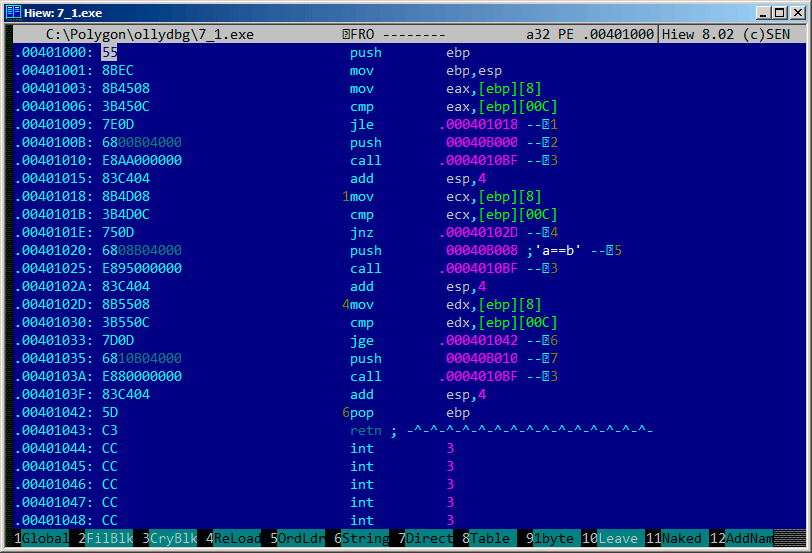
\includegraphics[scale=\FigScale]{patterns/07_jcc/simple/hiew_unsigned1.png}
\caption{Hiew: функция \TT{f\_unsigned()}}
\label{fig:jcc_hiew_1}
\end{figure}

Собственно, задач три:
\begin{itemize}
\item заставить первый переход срабатывать всегда;
\item заставить второй переход не срабатывать никогда;
\item заставить третий переход срабатывать всегда.
\end{itemize}

Так мы направим путь исполнения кода (code flow) во второй \printf,
и он всегда будет срабатывать и выводить на консоль \q{a==b}.

Для этого нужно изменить три инструкции (или байта):

\begin{itemize}
\item Первый переход теперь будет \JMP, но смещение перехода 
(\gls{jump offset}) останется прежним.

\item Второй переход может быть и будет срабатывать иногда, но в любом случае он будет совершать переход
только на следующую инструкцию, потому что мы выставляем смещение перехода (\gls{jump offset}) в 0.

В этих инструкциях смещение перехода просто прибавляется к адресу следующей инструкции.

Когда смещение 0, переход будет на следующую инструкцию.

\item Третий переход конвертируем в \JMP точно так же, как и первый, он будет срабатывать всегда.

\end{itemize}

\clearpage
Что и делаем:

\begin{figure}[H]
\centering
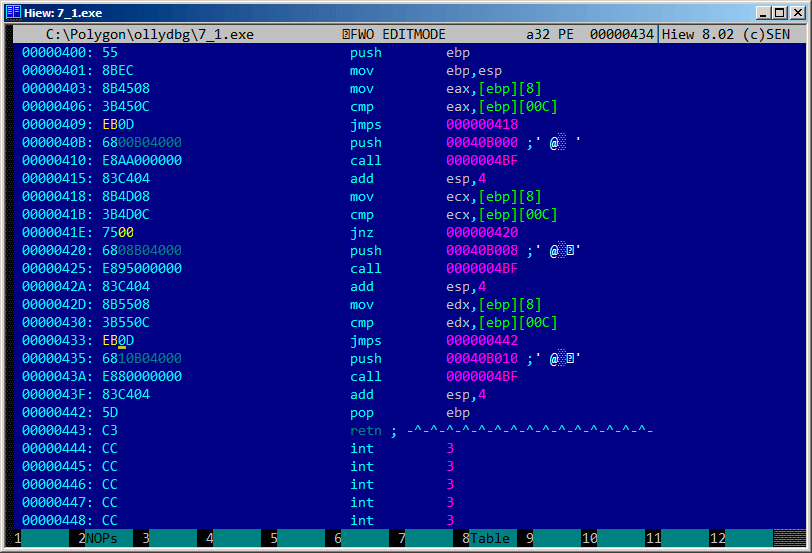
\includegraphics[scale=\FigScale]{patterns/07_jcc/simple/hiew_unsigned2.png}
\caption{Hiew: модифицируем функцию \TT{f\_unsigned()}}
\label{fig:jcc_hiew_2}
\end{figure}

Если забыть про какой-то из переходов, то тогда будет срабатывать несколько вызовов \printf, 
а нам ведь нужно чтобы исполнялся только один.

\subsubsection{\NonOptimizing GCC}

\myindex{puts() вместо printf()}
\NonOptimizing GCC 4.4.1 производит почти такой же код, за исключением \puts~(\myref{puts}) вместо \printf.

\subsubsection{\Optimizing GCC}

Наблюдательный читатель может спросить, зачем исполнять \CMP так много раз,
если флаги всегда одни и те же?
По видимому, оптимизирующий MSVC не может этого делать, но GCC 4.8.1 делает больше оптимизаций:

\lstinputlisting[caption=GCC 4.8.1 f\_signed()]{patterns/07_jcc/simple/GCC_O3_signed.asm}

% should be here instead of 'switch' section?
Мы здесь также видим \TT{JMP puts} вместо \TT{CALL puts / RETN}.
Этот прием описан немного позже: \myref{JMP_instead_of_RET}.

Нужно сказать, что x86-код такого типа редок.
MSVC 2012, как видно, не может генерировать подобное.
С другой стороны, программисты на ассемблере прекрасно осведомлены о том,
что инструкции \TT{Jcc} можно располагать последовательно.

Так что если вы видите это где-то, имеется немалая вероятность, что этот фрагмент кода был написан вручную.

Функция \TT{f\_unsigned()} получилась не настолько эстетически короткой:

\lstinputlisting[caption=GCC 4.8.1 f\_unsigned()]{patterns/07_jcc/simple/GCC_O3_unsigned_RU.asm}

Тем не менее, здесь 2 инструкции \TT{CMP} вместо трех.

Так что, алгоритмы оптимизации GCC 4.8.1, наверное, ещё пока не идеальны.
